\section{نتایج نسخه چندعاملی}
\label{sec:zs_results}
در این بخش، عملکرد الگوریتم‌ها در حالت چندعاملیِ بازی مجموع‌صفر ارائه و تحلیل می‌شود.

\subsection{توزیع پاداش تجمعی}
\begin{figure}[H]
	\centering
	
	% سطر اول
	\subfloat[شرایط اولیه تصادفی]{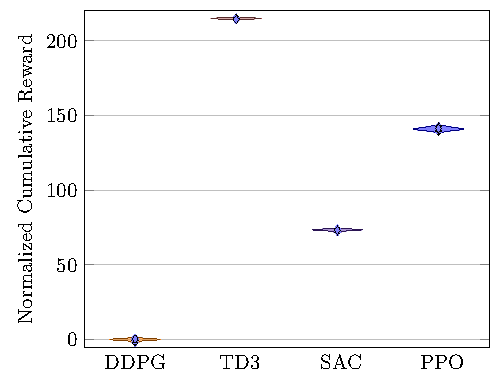
\includegraphics[width=.33\textwidth]{plots/ZeroSum/violin_plot/initial_condition_shift.pdf}}%
	\subfloat[اغتشاش در عملگرها]{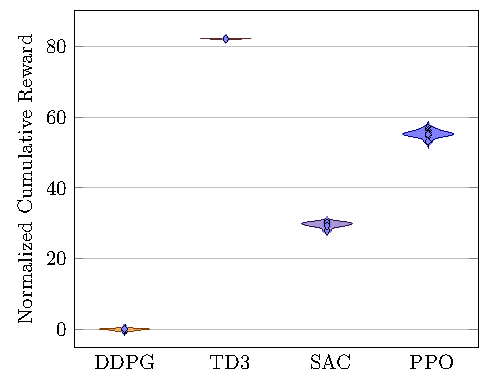
\includegraphics[width=.33\textwidth]{plots/ZeroSum/violin_plot/actuator_disturbance.pdf}}%
	\subfloat[عدم تطابق مدل]{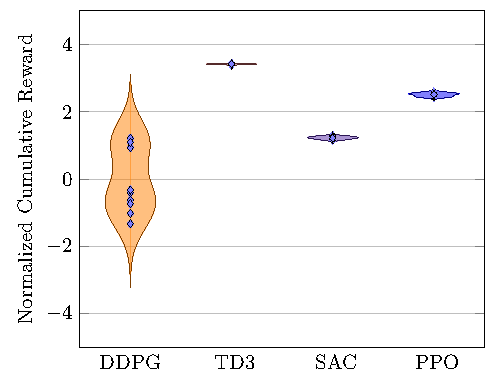
\includegraphics[width=.33\textwidth]{plots/ZeroSum/violin_plot/model_mismatch.pdf}}\\[1ex]
	
	% سطر دوم
	\subfloat[مشاهده ناقص]{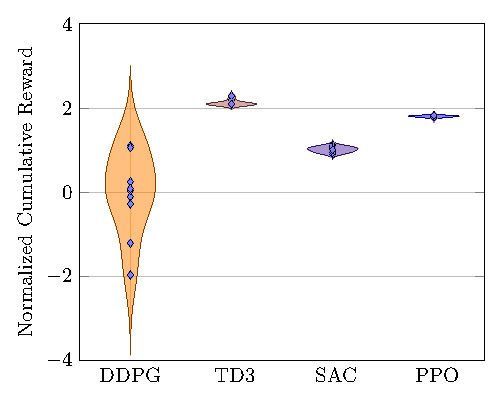
\includegraphics[width=.33\textwidth]{plots/ZeroSum/violin_plot/partial_observation.pdf}}%
	\subfloat[نویز حسگر]{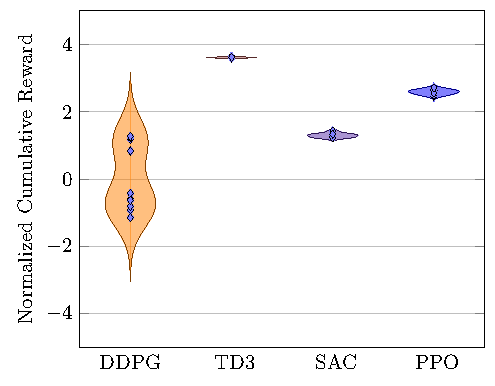
\includegraphics[width=.33\textwidth]{plots/ZeroSum/violin_plot/sensor_noise.pdf}}%
	\subfloat[تأخیر زمانی]{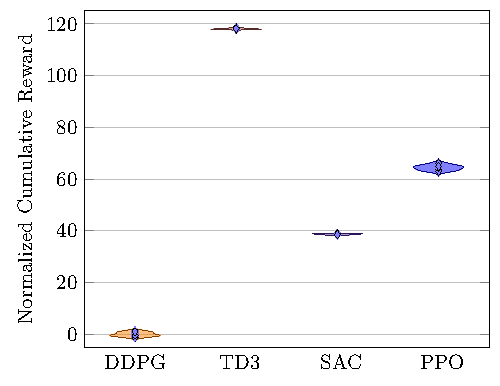
\includegraphics[width=.33\textwidth]{plots/ZeroSum/violin_plot/time_delay.pdf}}
	
	\caption{مقایسه توزیع پاداش تجمعی برای الگوریتم‌ها در حالت چندعاملی  در سناریوهای مختلف.}
	\label{fig:zs_robustness_violin}
\end{figure}

\subsection{مقایسه عددی}
\begin{table}[H]
	\centering
	\setlength{\tabcolsep}{6pt}      % tighter columns (built-in)
	\renewcommand{\arraystretch}{1.5}% a bit more row height (built-in)
	\scriptsize                      % smaller font to fit
	
	% --- Row 1: left + right boxes, centered as a group ---
	\makebox[\linewidth][c]{%
		\parbox{.48\linewidth}{
			\centering
			\footnotesize
			\begin{tabular}{@{} R {2.6cm}*{4}{c}}
				\toprule
				{سناریو} & \lr{DDPG} & \lr{PPO} & \lr{SAC} & \lr{TD3} \\
				\midrule
				شرایط اولیه تصادفی & $-0.41$ & $0.34$ & $-0.02$ & ${0.74}$ \\
				اغتشاش در عملگرها & $-0.44$ & $0.35$ & $-0.02$ & ${0.73}$ \\
				عدم تطابق مدل      & $-0.63$ & $0.38$ & $-0.13$ & ${0.75}$ \\
				مشاهده ناقص        & $-1.52$ & $0.40$ & $-0.44$ & ${0.71}$ \\
				نویز حسگر          & $-0.60$ & $0.37$ & $-0.12$ & ${0.75}$ \\
				تأخیر زمانی        & $-1.19$ & $0.17$ & $-0.05$ & ${0.67}$ \\
				\bottomrule
			\end{tabular}
			\caption*{\normalfont پاداش تجمعی}
		}
		\hspace{0.04\linewidth}
		\parbox{.48\linewidth}{
			\centering
			\footnotesize
			\begin{tabular}{@{} R {2.6cm}*{4}{c}}
				\toprule
				{سناریو} & \lr{DDPG} & \lr{PPO} & \lr{SAC} & \lr{TD3} \\
				\midrule
				شرایط اولیه تصادفی & $4.42$ & $4.30$ & $4.02$ & ${1.22}$ \\
				اغتشاش در عملگرها & $4.39$ & $4.38$ & $4.01$ & ${1.26}$ \\
				عدم تطابق مدل      & $8.85$ & $3.57$ & $4.78$ & ${1.25}$ \\
				مشاهده ناقص        & $9.65$ & $2.44$ & $5.17$ & ${1.09}$ \\
				نویز حسگر          & $9.12$ & $3.58$ & $4.66$ & ${1.25}$ \\
				تأخیر زمانی        & $6.73$ & $4.53$ & $4.12$ & ${1.21}$ \\
				\bottomrule
			\end{tabular}
			\caption*{\normalfont مجموع خطای مسیر}
		}%
	}
	
	\vspace{0.6em}
	
	% --- Row 2: left + right boxes, centered as a group ---
	\makebox[\linewidth][c]{%
		\parbox{.48\linewidth}{
			\centering
			\footnotesize
			\begin{tabular}{@{} R {2.6cm}*{4}{c}}
				\toprule
				{سناریو} & \lr{DDPG} & \lr{PPO} & \lr{SAC} & \lr{TD3} \\
				\midrule
				شرایط اولیه تصادفی & $5.11$ & ${0.77}$ & $1.76$ & $3.31$ \\
				اغتشاش در عملگرها & $4.89$ & ${0.77}$ & $1.71$ & $3.07$ \\
				عدم تطابق مدل      & $5.48$ & ${0.86}$ & $2.37$ & $4.32$ \\
				مشاهده ناقص        & $5.37$ & ${1.03}$ & $2.33$ & $4.10$ \\
				نویز حسگر          & $5.48$ & ${0.86}$ & $2.37$ & $4.30$ \\
				تأخیر زمانی        & $5.51$ & ${0.76}$ & $2.11$ & $5.12$ \\
				\bottomrule
			\end{tabular}
			\caption*{\normalfont مجموع تلاش کنترلی}
		}
		\hspace{0.04\linewidth}
		\parbox{.48\linewidth}{
			\centering
			\footnotesize
			\begin{tabular}{@{} R {2.6cm}*{4}{c}}
				\toprule
				{سناریو} & \lr{DDPG} & \lr{PPO} & \lr{SAC} & \lr{TD3} \\
				\midrule
				شرایط اولیه تصادفی & $0.00$ & $0.00$ & $0.00$ & $0.00$ \\
				اغتشاش در عملگرها & $0.00$ & $0.00$ & $0.00$ & $0.00$ \\
				عدم تطابق مدل      & $0.00$ & $0.00$ & $0.20$ & $0.00$ \\
				مشاهده ناقص        & $0.00$ & $0.00$ & $0.20$ & $0.00$ \\
				نویز حسگر          & $0.00$ & $0.00$ & $0.20$ & $0.00$ \\
				تأخیر زمانی        & $0.00$ & $0.00$ & $0.20$ & $0.00$ \\
				\bottomrule
			\end{tabular}
			\caption*{\normalfont احتمال شکست}
		}%
	}
	
	\caption{مقایسه الگوریتم‌های چندعاملی در سناریوهای مختلف مقاومت}
\end{table}

%\subsection{تحلیل و بحث}
در حالت چندعاملی، \lr{TD3}
  به‌طور پایدار پاداش بالاتر و خطای مسیر کمتر ثبت می‌کند، در حالی‌که \lr{PPO} کمترین تلاش کنترلی را نشان می‌دهد. عملکرد \lr{SAC} و \lr{DDPG} در برخی سناریوهای دشوار ضعیف‌تر است، هرچند نرخ‌های شکست عمدتاً پایین باقی می‌ماند.